\chapter{NP}

\section{Complexiteit: P en NP}
\begin{figure}[ht]
    \centering
    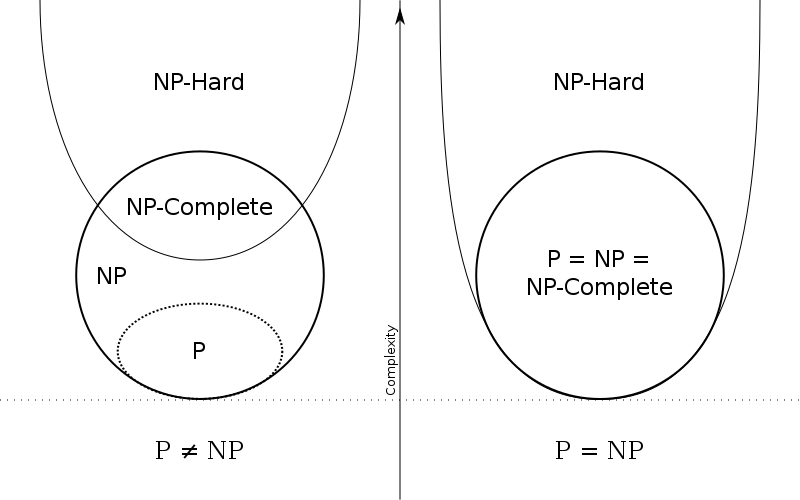
\includegraphics[width=\textwidth]{P_vs_NP}
    \caption{De linkse deelfiguur toont de verschillende complexiteitsklassen indien $P \neq NP$. De rechtse deelfiguur toont hetzelfde indien $P = NP$.}
    \label{fig:P_vs_NP}
\end{figure}

\begin{itemize}
    \item Alle besproken algoritmen hebben een efficiënte oplossing. 
    \item Hun uitvoeringstijd wordt begrensd door een \textbf{veelterm} zoals $O(n^2)$ of $O(n^2m)$.
    \item Sommige problemen hebben hebben geen efficiënte oplossing.
    \item Problemen worden onderverdeeld in \textbf{complexiteitsklassen}.
    \begin{itemize}
        \item Beperking tot  \textbf{beslissingsproblemen}, waarbij de uitvoer \textit{ja} of \textit{nee} is.
        \item Niet echt een beperking omdat elk probleem als een beslissingsproblemen kan geformuleerd worden.
    \end{itemize}
\end{itemize}

\subsection{Complexiteitsklassen}
\begin{itemize}
    \item De klasse \textbf{P} (\textbf{P}olynomiaal) bevat alle problemen waarvan de uitvoeringstijd begrensd wordt door een veelterm.
    \begin{itemize}
        \item Op een realistisch computermodel.
        \begin{itemize}
            \item Heeft een polynomiale bovengrens voor het werk dat in één tijdseenheid kan verricht worden.
        \end{itemize}
        \item Met een redelijke voorstelling van de invoergegevens (geen overbodige informatie, compact, ...).
        \item Al de problemen in \textbf{P} worden als efficiënt oplosbaar beschouwd.
        \alert Waarom een veelterm? $O(n^{100})$ kan nauwelijks efficiënt genoemd worden.
        \begin{enumerate}
            \item Meestal is de graad van de veelterm beperkt tot twee of drie.
            \item Veeltermen vormen de kleinste klasse functies die kunnen gecombineerd worden, en opnieuw een veelterm opleveren.
            \begin{itemize}
                \item Men noemt dit een \textbf{gesloten klasse}.
                \item Efficiënte algoritmen voor eenvoudigere problemen kunnen dus gecombineerd worden tot een efficiënt algoritme voor een complex probleem.
            \end{itemize}
            \item De efficiëntiemaat blijft onafhankelijk van het computermodel.
        \end{enumerate}
    \end{itemize}
    \item De klasse \textbf{NP} (\textbf{N}iet-deterministisch \textbf{P}olynomiaal) bevat alle problemen die door een niet-deterministische computer in polynomiale tijd kunnen opgelost worden en waarvan de oplossing kan gecontroleerd worden in polynomiale tijd.
    \begin{itemize}
        \item Een niet-deterministische computer bevat hypothetisch een oneindig aantal processoren, waarvan er op tijdstap $t$ er $k$ kunnen aangesproken van worden. De processoren werken niet samen, maar kunnen wel hun deel van het probleem oplossen.
        \item Elk probleem uit \textbf{P} behoort tot \textbf{NP}. 
        \item Niet geweten of er probleem in \textbf{NP} zit die niet tot \textbf{P} behoort $\rightarrow \textbf{P}$ vs $\textbf{NP}$ probleem (Figuur \ref{fig:P_vs_NP}). 
        \item Wel geweten dat er problemen zijn die niet in \textbf{NP} zitten, en dus ook niet in \textbf{P}.
    \end{itemize}
    \item De klasse \textbf{NP-hard} bevat alle problemen die minstens even zwaar zijn als elk \textbf{NP}-probleem.
    \begin{itemize}
        \item Een probleem $X$ dat gereduceerd kan worden naar een probleem $Y$ betekent dat $Y$ minstens even zwaar is als $X$.
    \end{itemize}
    \item De klasse \textbf{NP-compleet} bevat alle problemen die \textbf{NP-hard} zijn, maar toch nog in \textbf{NP} zitten.
    \begin{itemize}
        \item Als er één \textbf{NP-compleet} probleem bestaat die efficiënt oplosbaar zou zijn (en dus in \textbf{P} behoort), dan zouden alle problemen uit \textbf{NP} ook efficiënt oplosbaar zijn, zodat $\textbf{P} = \textbf{NP}$.
        \item NP-complete problemen kunnen op verschillende manieren aangepakt worden:
        \begin{itemize}
            \item Backtracking en snoeien.
            \item Speciale gevallen oplossen met efficiënte algoritmen.
            \item Het kan zijn dat de gemiddelde uitvoeringstijd toch goed is.
            \item Gebruik een benaderend algoritme.
            \item Maak gebruik van heuristieken.
        \end{itemize}
    \end{itemize}
    
\end{itemize}

\section{NP-complete problemen}

\begin{itemize}
    \item Overzicht van belangrijke NP-complete (optimalisatie)problemen.
    \item Om na te gaan of een probleem NP-compleet is, moet het herleid kunnen worden naar een basisvorm.
\end{itemize}

\subsection{Het basisprobleem: SAT (en 3SAT)}
\begin{itemize}
    \item Gegeven:
    \begin{itemize}
        \item Een verzameling logische variabelen $\mathcal{X} = \{x_1, \dots, x_{|\mathcal{X}|}\}$.
        \item Een verzameling logische uitspraken $\mathcal{F} = \{f_1, \dots, f_{|\mathcal{F}|}\}$.
        \item Elke uitspraak bestaat uit automaire uitspraken (atomen) samengevoegd met OF-operaties:
        $$f_1 = x_2 \vee \overline{x_5} \vee x_7 \vee x_8$$
    \end{itemize}
    \item Gevraagd:
    \begin{itemize}
        \item  Hoe moeten de waarden toegekend worden aan de variabelen uit $\mathcal{X}$ zodat elke uitspraak in $\mathcal{F}$ waar is?
    \end{itemize}
    \item Elk NP-compleet probleem is reduceerbaar tot SAT.
    \item Een uitspraak met meer dan drie atomen kan herleidt worden naar een reeks uitspraken met elk drie atomen:
    \begin{align*}
        f_1 = &x_2 \vee \overline{x_5} \vee x_n \\
        f_1' = &\overline{x_n} \vee x_7 \vee x_8
    \end{align*}
\end{itemize}

\subsection{Vertex Cover}
\begin{itemize}
    \item Gegegeven:
    \begin{itemize}
        \item Een ongerichte graaf.
    \end{itemize}
    \item Gevraagd:
    \begin{itemize}
        \item Hoe kan de kleinste groep knopen bepaald worden die minsten één eindknoop van elke verbinding bevat.
    \end{itemize}

    \item Voorbeeld:
    \begin{itemize}
        \item 3SAT kan gereduceerd worden tot vertex cover.
        \begin{itemize}
            \item Voor elke logische variabele $x_i$ worden er twee knopen gemaakt: voor $x_i$ en $\overline{x}_i$. Deze knopen zijn verbonden.
            \item Voor elke uitspraak worden er drie knopen gemaakt, één voor elk atoom. Deze drie knopen worden verbonden. Elk atoom wordt ook verbonden met de knopen voor de individuele logische variabelen.
        \end{itemize}
        \item Voor elke logische variabele moet zeker één van de twee knopen opgenomen worden.
        \item Voor elke uitspraak moeten zeker twee van de drie knopen opgenomen worden.
        \item Minstens $|\mathcal{X}| + 2|\mathcal{F}|$ knopen.
        \item Stel volgende uitspraken 

        \begin{align*}
            U_1 = \overline{x}_1 \vee x_2 \vee x_3 \\
            U_2 = x_2 \vee \overline{x}_3 \vee x_4
        \end{align*}

        Bijhorende graaf:
        \begin{figure}[ht]
            \centering
            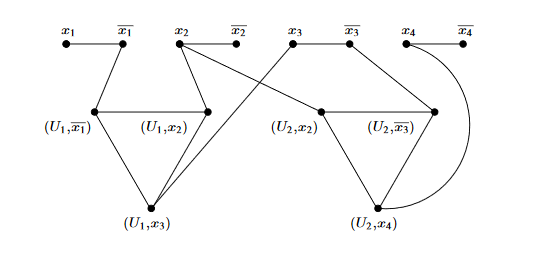
\includegraphics[width=0.5\textwidth]{vertex_cover}
            \caption{Een graaf voor het 3SAT-probleem.}
            \label{fig:vertex_cover}
        \end{figure}

        Voorbeeld van een minimale vertex cover:
        \begin{figure}[ht]
            \centering
            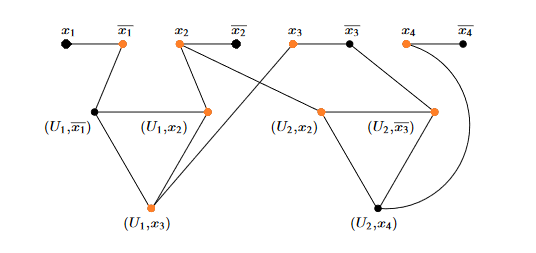
\includegraphics[width=0.5\textwidth]{vertex_cover_solved}
            \caption{Een minimale vertex cover van de graaf op figuur \ref{fig:vertex_cover}}
            \label{fig:vertex_cover_solved}
        \end{figure}
    \end{itemize}
    \item Andere voorbeelden van minimale vertex covers:
    \begin{figure}[ht]
        \centering
        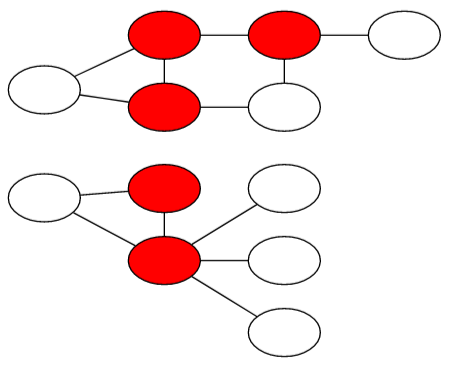
\includegraphics[width=0.5\textwidth]{minimum_vertex_cover}
        \caption{De minimale vertex cover van twee verschillende grafen.}
        \label{fig:minimum_vertex_cover}
    \end{figure}
\end{itemize}

\subsection{Dominating set}
\begin{itemize}
    \item Gegeven:
    \begin{itemize}
        \item Een ongerichte graaf.
    \end{itemize}
    \item Gevraagd:
    \begin{itemize}
        \item Een kleinste groep knopen zodat elke andere knoop met minstens een van de knopen uit de groep verbonden is.
    \end{itemize}
    \item Voorbeelden:
    \begin{figure}[ht]
        \centering
        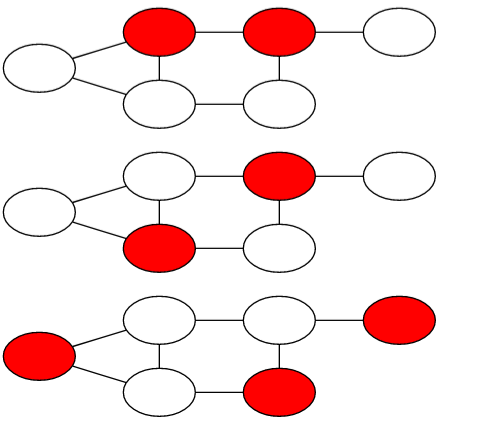
\includegraphics[width=0.5\textwidth]{dominating_set}
        \caption{Voorbeelden van dominating sets.}
        \label{fig:dominating_set}
    \end{figure}
\end{itemize}

\subsection{Graph Coloring}
\begin{itemize}
    \item \textbf{Vertex coloring}:
    \begin{itemize}
        \item Gegeven:
        \begin{itemize}
            \item Een ongerichte graaf.
        \end{itemize}
        \item Gevraagd:
        \begin{itemize}
            \item Kleur de knopen met een minimum aantal kleuren, zodat de eindknopen van elke verbinding een verschillende kleur hebben.
        \end{itemize}
        \item Voorbeeld:
        \begin{figure}[ht]
            \centering
            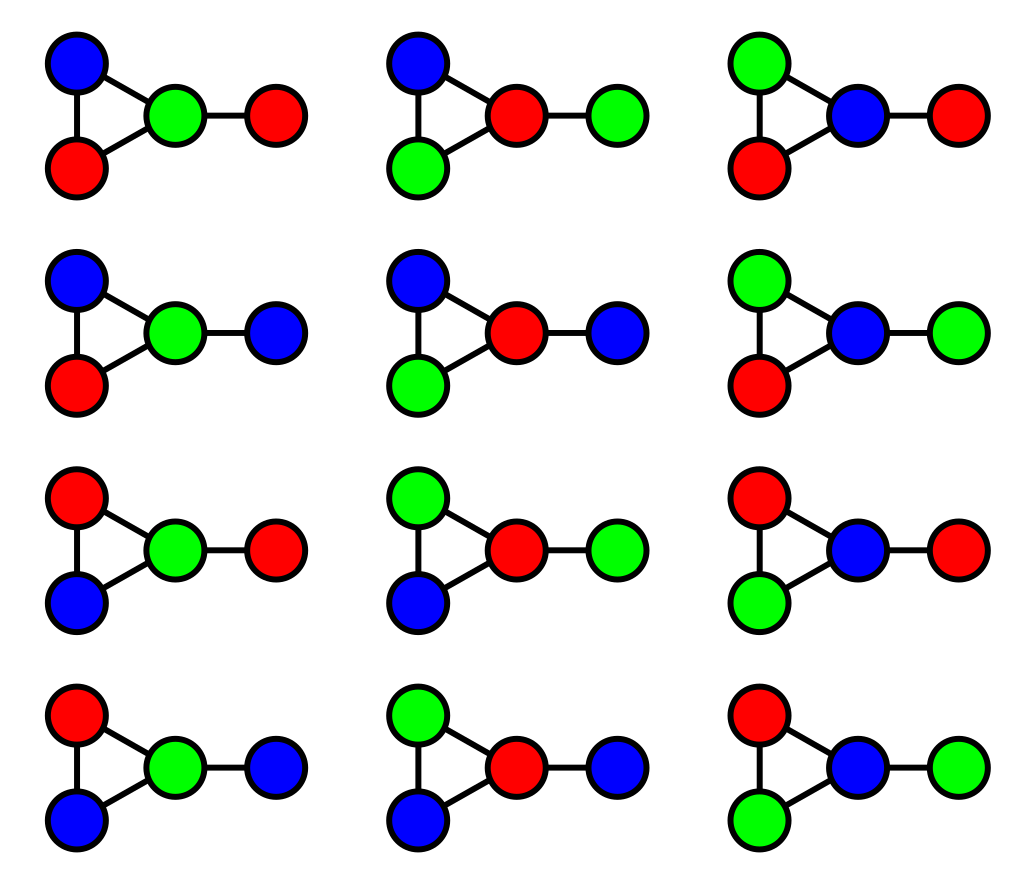
\includegraphics[width=0.25\textwidth]{vertex_coloring}
            \caption{De knopen van een graaf kunnen op meerdere manieren gekleurd worden.}
            \label{fig:vertex_coloring}
        \end{figure}
    \end{itemize}

    \item \textbf{Edge coloring}:
    \begin{itemize}
        \item Gegeven:
        \begin{itemize}
            \item Een ongerichte graaf.
        \end{itemize}
        \item Gevraagd:
        \begin{itemize}
            \item Kleur de verbindingen met een minimum aantal kleuren, zodat verbindingen met dezelfde eindknoop een verschillende kleur hebben.
        \end{itemize}
        \item Voorbeeld:
        \begin{figure}[ht]
            \centering
            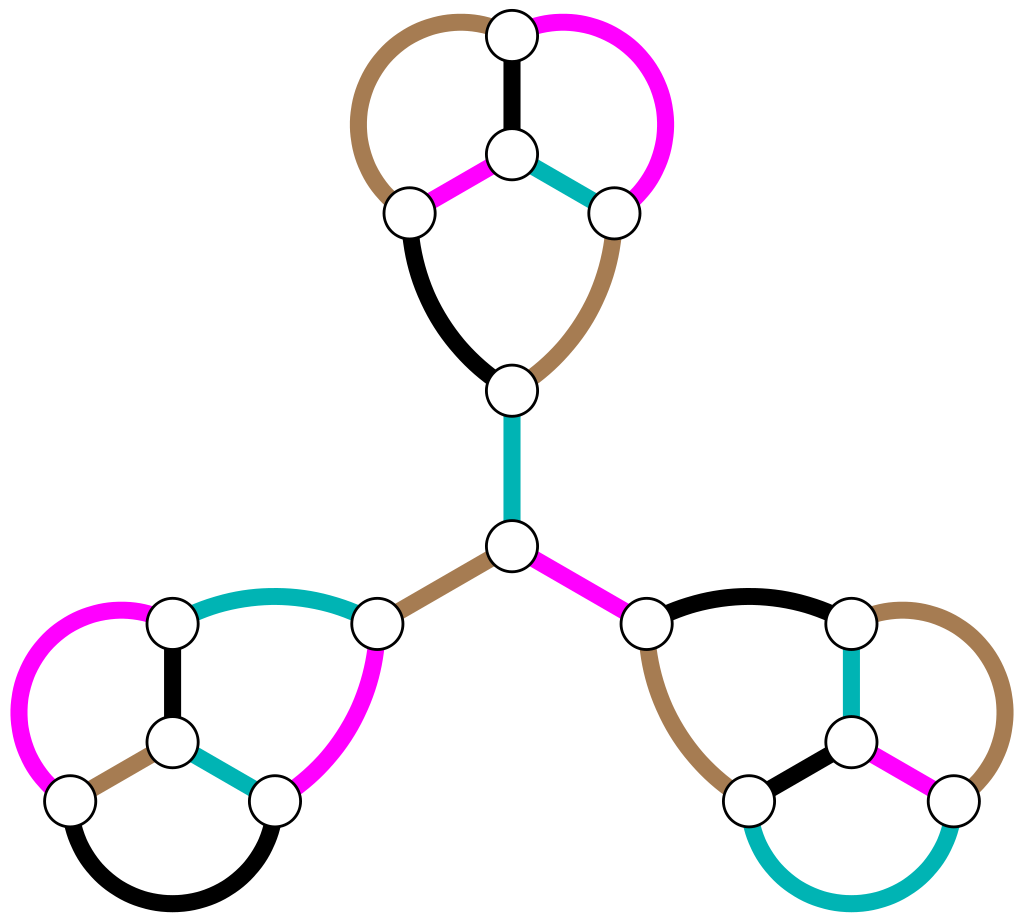
\includegraphics[width=0.25\textwidth]{edge_coloring}
            \caption{Elke knoop heeft graad 3 dus zijn er hoogstens 4 kleuren nodig om de verbindingen te kleuren.}
            \label{fig:edge_coloring}
        \end{figure}
    \end{itemize}
    
\end{itemize}


\subsection{Clique}
\begin{itemize}
    \item Gegeven:
    \begin{itemize}
        \item Een ongerichte graaf.
    \end{itemize}
    \item Gevraagd:
    \begin{itemize}
        \item De grootste groep knopen die allemaal met elkaar verbonden zijn.
    \end{itemize}
    \item Voorbeeld:
    \begin{figure}[ht]
        \centering
        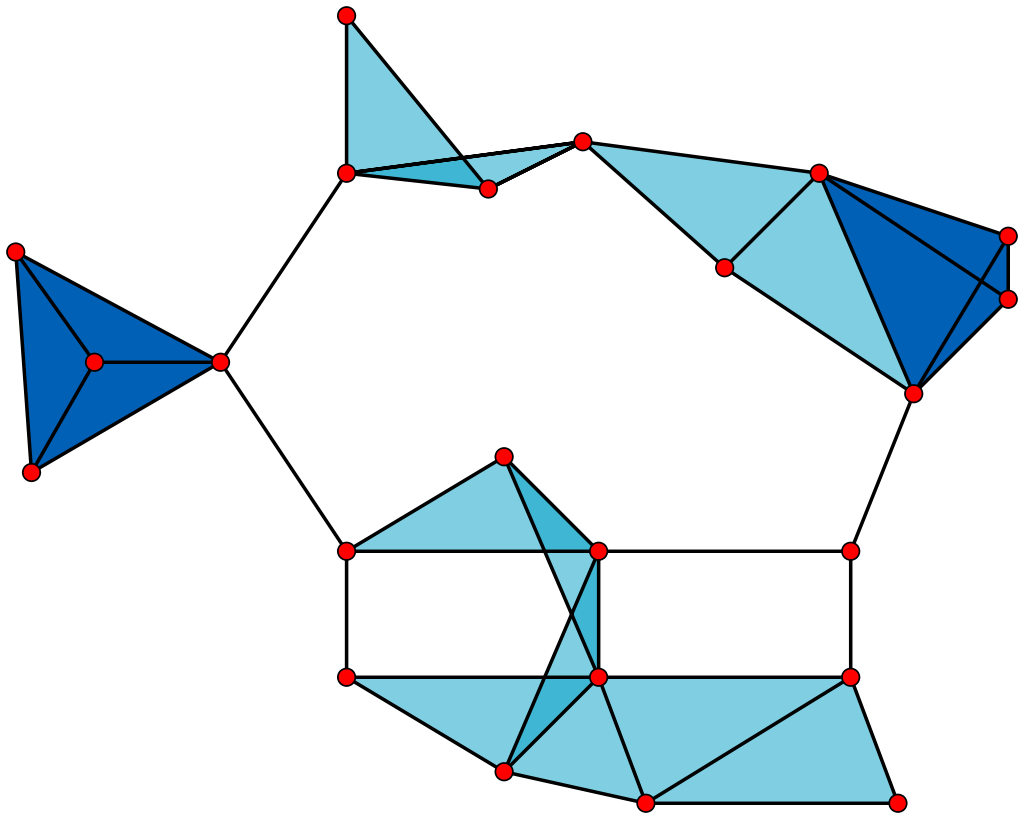
\includegraphics[width=0.5\textwidth]{clique}
        \caption{Deze graaf bevat 23 1-knoop cliques (de knopen), 49 2-knoop cliques (door de verbindingen), 19 3-knoop cliques (lichtblauwe driehoeken) en 2 4-knoop cliques (donkerblauwe oppervlakken). In deze graaf zijn de twee 4-knoop de grootste groep van knopen.}
        \label{clique}
    \end{figure}
    \begin{itemize}
        \item Het SAT probleem kan herleidt worden tot clique.
        \begin{itemize}
            \item Voor elk voorkomen van een atoom in een uitspraak wordt twee knopen $(F_i, x_j)$ en $(F_i, \overline{x_j})$ aangemaakt.
            \item Er is een verbinding tussen knopen die horen bij verschillende uitspraken als de atomen elkaar niet uitsluiten:
            \begin{itemize}
                \item $(F_i, x_k)$ met $(F_j, x_l)$ voor alle $k$ en $l$.
                \item $(F_i, \overline{x_k})$ met $(F_i, \overline{x_l})$ voor alle $k$ en $l$.
                \item $(F_i, x_k)$ met $(F_i, \overline{x_l})$ als $k \neq l$.
            \end{itemize}
        \end{itemize}
        \item Een clique kan hoogstens $|\mathcal{F}|$ elementen bevatten.
    \end{itemize}
\end{itemize}

\subsection{Independent set}
\begin{itemize}
    \item Gegeven:
    \begin{itemize}
        \item Een ongerichte graaf.
    \end{itemize}
    \item Gevraagd:
    \begin{itemize}
        \item De grootste groep knopen zonder gemeenschappelijke verbindingen.
    \end{itemize}
    \item Voorbeeld:
    \begin{figure}[ht]
        \centering
        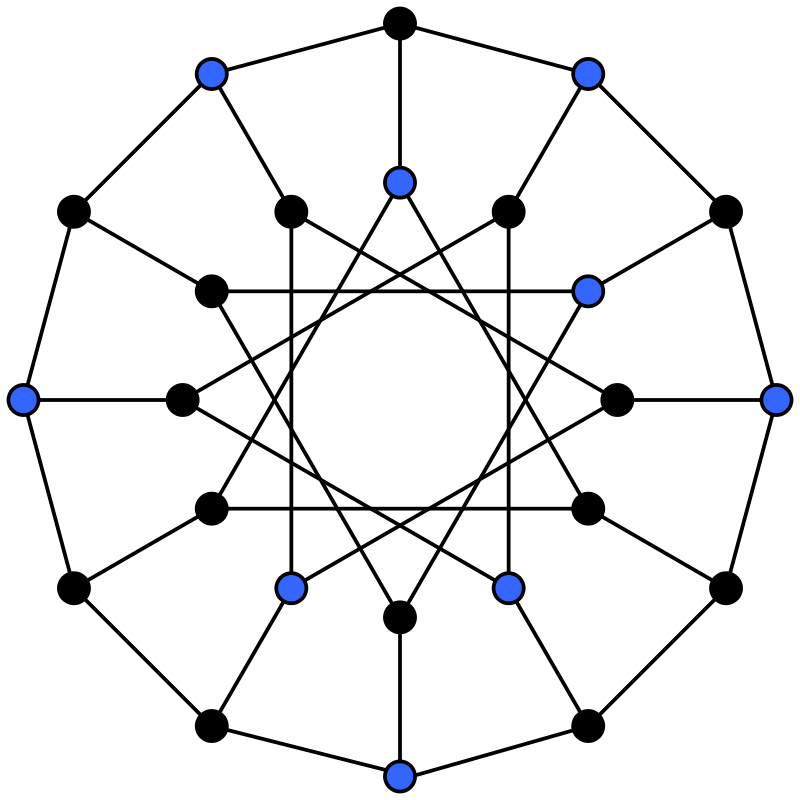
\includegraphics[width=0.5\textwidth]{independent_set}
        \caption{De blauwe knopen vormen de independent set.}
        \label{fig:independent_set}
    \end{figure}

\end{itemize}

\subsection{Hamilton path}
\begin{itemize}
    \item Gegeven:
    \begin{itemize}
        \item Een al dan niet gerichte graaf.
    \end{itemize}
    \item Gevraagd:
    \begin{itemize}
        \item Bestaat er een circuit dat elke knoop eenmaal bevat?
    \end{itemize}
    \item Voorbeeld:
    \begin{figure}[ht]
        \centering
        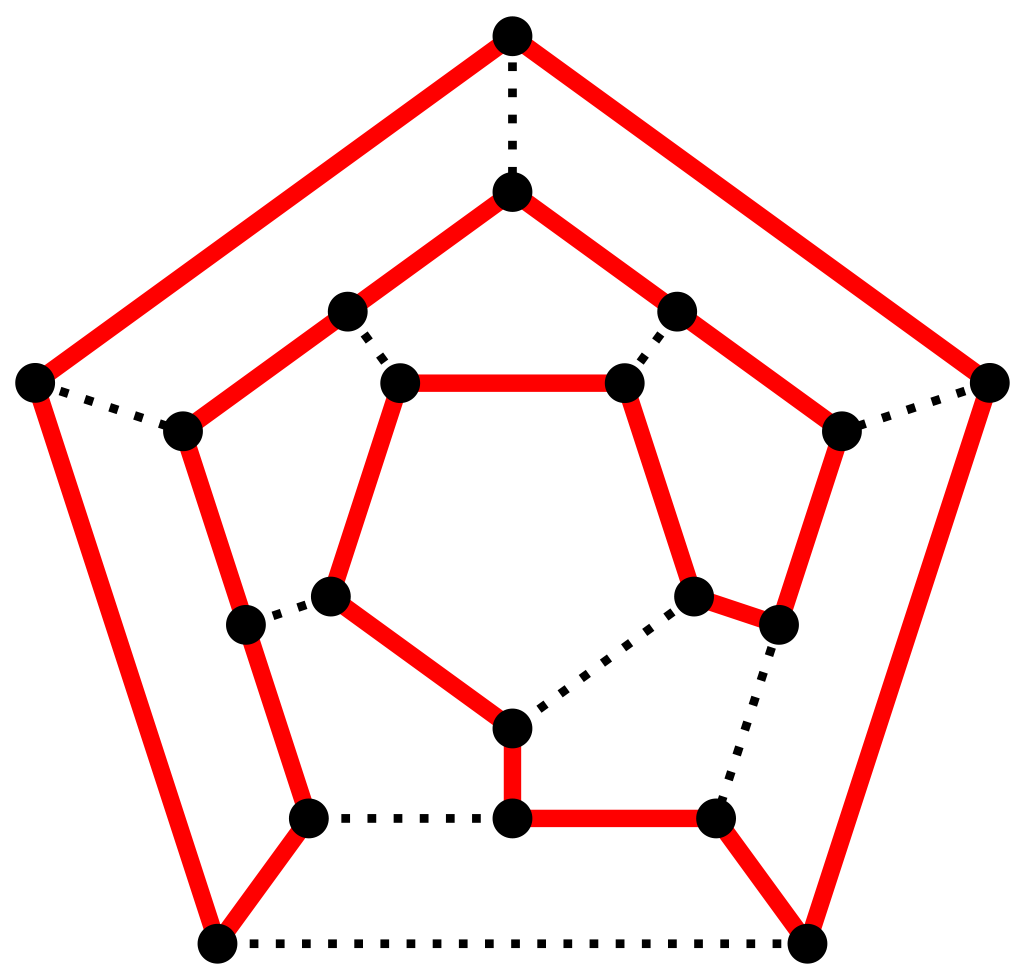
\includegraphics[width=0.5\textwidth]{hamilton_path}
        \caption{Een tweedimensionale weergave van een Hamiltonpad door een dodecaëder. De zwarte stippelijnen zijn ook verbindingen.}
        \label{fig:hamilton_path}
    \end{figure}

\end{itemize}

\subsection{Minimum cover}
\begin{itemize}
    \item Gegeven:
    \begin{itemize}
        \item Een verzameling $\mathcal{S}$.
        \item Een collectie deelverzamelingen $\mathcal{C}$ van $\mathcal{S}$.
    \end{itemize}
    \item Gevraagd:
    \begin{itemize}
        \item De kleinste deelverzameling $\mathcal{C}'$ van $\mathcal{C}$ zodat elk element van $\mathcal{S}$ tot minstens één van de deelverzamelingen uit $\mathcal{C}'$ behoort.
    \end{itemize}
    \item Voorbeeld:
    \begin{itemize}
        \item Dit kan efficiënt opgelost worden als de deelverzamelingen in $\mathcal{C}$ niet meer dan twee elementen bevatten.                      
        \item Als elke $C \in \mathcal{C}$ exact twee elementen heeft is het equivalent met edge cover.
        \item Als er $C \in \mathcal{C}$ zijn met slechts één element kunnen deze geschrapt worden en dan edge cover oplossen.
        \item SAT kan ook herleidt worden tot minimum cover.
        \begin{itemize}
            \item Neem $\mathcal{S} = \mathcal{F} \cup \mathcal{X}$
            \item Voor elke logische variabele $x_i$ zijn er twee elementen van $C$
            \begin{align*}
                C_{x_i} &= \{x_i \} \cup \{F \in \mathcal{F} : x_i \in F \}\\
                C_{\overline{x_i}} &= \{x_i \} \cup \{F \in \mathcal{F} : \overline{x_i} \in F \}
            \end{align*}
        \end{itemize}
    \end{itemize}
\end{itemize}

\subsection{Subset sum}
\begin{itemize}
    \item Gegeven:
    \begin{itemize}
        \item Een verzameling elementen met elk een positieve gehele grootte.
        \item Een positief geheel getal $k$.
    \end{itemize}
    \item Gevraagd:
    \begin{itemize}
        \item Een deelverzameling van die elementen, zodat de som van hun grootten gelijk is aan $k$.
    \end{itemize}
\end{itemize}

\subsection{Partition}
\begin{itemize}
    \item Gegeven:
    \begin{itemize}
        \item Een zak van positieve gehele getallen.
    \end{itemize}
    \item Gevraagd:
    \begin{itemize}
        \item Kan die opgesplitst worden in twee deelverzamelingen, zodat de som van de grootten van de ene gelijk is aan de som van de grootten van de andere.
    \end{itemize}
\end{itemize}

\subsection{Travelling salesman problem}
\begin{itemize}
    \item Gegeven:
    \begin{itemize}
        \item Een aantal steden, en de afstand tussen elk paar steden.
    \end{itemize}
    \item Gevraagd:
    \begin{itemize}
        \item Het kortste circuit dat elke stad eenmaal bevat.
    \end{itemize}
\end{itemize}

\subsection{Longest path}
\begin{itemize}
    \item Gegeven:
    \begin{itemize}
        \item Een gerichte of ongerichte gewogen graaf.
        \item Twee knopen $s$ en $t$.
    \end{itemize}
    \item Gevraagd:
    \begin{itemize}
        \item De langste weg zonder lussen van $s$ naar $t$.
    \end{itemize}
\end{itemize}

\subsection{Bin packing}
\begin{itemize}
    \item Gegeven:
    \begin{itemize}
        \item Een verzameling van $n$ objecten met afmetingen $s_1, \cdots, s_n$.
        \item Een verzameling van $m$ bakken met capaciteiten $c_1, \cdots, c_m$.
    \end{itemize}
    \item Gevraagd:
    \begin{itemize}
        \item Sla alle objecten op in zo weinig mogelijk bakken 
    \end{itemize}
\end{itemize}

\subsection{Knapsack}
\begin{itemize}
    \item Gegeven:
    \begin{itemize}
        \item Een verzameling van $n$ objecten met elk een afmeting.
        \item Een knapzak met een zekere capaciteit.
    \end{itemize}
    \item Gevraagd:
    \begin{itemize}
        \item Steek objecten in de zak zonder zijn capaciteit te overschrijden, zodat hun totale waarde zo groot mogelijk is.
    \end{itemize}
\end{itemize}